\documentclass[10pt]{article}
\usepackage[margin=0.72in]{geometry}
\usepackage{graphicx}
\usepackage{booktabs}
\usepackage{longtable}
\usepackage{array}
\usepackage{tabularx}
\usepackage{xurl}
\usepackage{hyperref}
\usepackage{enumitem}
\urlstyle{same}
\hypersetup{breaklinks=true}
\setlist{nosep,leftmargin=*}
\setlength{\parskip}{0.35em}
\setlength{\tabcolsep}{4pt}
\renewcommand{\arraystretch}{1.18}
\setlength{\extrarowheight}{1.2pt}
\setlength{\LTpre}{0.55em}
\setlength{\LTpost}{0.55em}
\setlength{\emergencystretch}{3em}
\newcolumntype{L}[1]{>{\raggedright\arraybackslash}p{#1}}
\newcolumntype{Y}{>{\raggedright\arraybackslash}X}

\title{Axiom Shopping Assistant: CIS 5500 Final Report}
\author{Chenguang Shen, Luis Garcia, Leo Tan, Anika Madan}
\date{Spring 2026}

\begin{document}
\maketitle

\section{Introduction}
Axiom is a full-stack shopping analytics application over large Amazon product
and review data. The target problem is information overload: product pages show
prices, star ratings, review counts, and seller labels, but shoppers still have
to do the hard work of comparing alternatives, estimating whether a deal is
meaningful, and deciding which review signals are trustworthy. Axiom turns those
signals into searchable product discovery, product-detail evidence, cart
savings, category and brand analytics, and a customizable value ranking.

The application was built by Chenguang Shen, Luis Garcia, Leo Tan, and Anika
Madan. Our main goals were:
\begin{itemize}
  \item integrate overlapping product, category, brand, user, and review/comment
  data into a normalized PostgreSQL schema;
  \item expose the data through robust Express API routes with input validation
  and stable JSON response shapes;
  \item build a React/Vite frontend with multiple distinct pages that all read
  from the database-backed API; and
  \item preserve original and optimized SQL paths so performance gains from
  indexing, caching, query restructuring, and materialized views are measurable.
\end{itemize}

The final interface includes a visible query-mode toggle. In standard mode the
client calls original SQL paths; in optimized mode it appends
\texttt{?optimized=1}, letting the backend choose optimized SQL or cached
responses without changing the public API.

\section{Architecture and Application Functionality}
The system has three tiers. The frontend is a React/Vite single-page
application, the backend is an Express server using the Node \texttt{pg} pool,
and the database is PostgreSQL hosted on AWS RDS. The data pipeline is written
in Python with pandas and psycopg2; operational SQL and benchmark scripts live
under \texttt{database/} and \texttt{scripts/}.

\begin{center}
\begin{tabularx}{\linewidth}{@{}L{0.16\linewidth}L{0.27\linewidth}Y@{}}
\toprule
Layer & Technologies & Responsibility \\
\midrule
Client & React, Vite, React Router & Pages, filters, charts, cart state \\
API & Node.js, Express, \texttt{pg} & Validation, caching, route contracts \\
Database & PostgreSQL on AWS RDS & Normalized tables, indexes, materialized views \\
Data tools & Python, pandas, psycopg2 & Cleaning, entity resolution, ingestion \\
Testing/ops & Vitest, Supertest, benchmark scripts & Regression tests and timings \\
\bottomrule
\end{tabularx}
\end{center}

\subsection{Pages}
The application has multiple database-backed pages with distinct workflows:
\begin{itemize}
  \item \textbf{Home} provides a search entry point, featured proven picks from
  recent review activity, and discounted products.
  \item \textbf{Browse} supports keyword search, category discovery, category
  preview cards, and post-Milestone-4 category/brand product-list pages with
  URL-backed filters.
  \item \textbf{Deals} ranks discounted products by percentage off, with price
  and rating filters.
  \item \textbf{Category and Brand pages} paginate products for one category or
  brand and keep filters in the URL.
  \item \textbf{Product Detail} shows product metadata, rating distribution,
  reviewer context, cheaper higher-rated alternatives, and cart actions.
  \item \textbf{Cart} persists selected products in local storage and posts ASINs
  to the backend for live savings aggregation.
  \item \textbf{Analytics} visualizes category comparison, brand performance, and
  monthly review trends by reviewer activity group.
  \item \textbf{Value Rankings} lets users weight rating strength, review depth,
  price efficiency, and recent review activity. The Balanced preset uses
  \texttt{0.4/0.2/0.2/0.2}, matching the indexed default score in the optimized
  materialized view.
\end{itemize}

\section{Data}
The final database integrates product metadata with two review/comment sources:
\begin{itemize}
  \item \textbf{Amazon Products 2023.} We use the Amazon product and category
  catalog released on Kaggle by asaniczka:
  \href{https://www.kaggle.com/datasets/asaniczka/amazon-products-dataset-2023-1-4m-products}{Amazon Products Dataset 2023}. It provides ASINs, titles, image URLs,
  product URLs, prices, list prices, star ratings, review counts, best-seller
  flags, and category IDs.
  \item \textbf{Original Amazon review/comment export.} The checked-in
  \texttt{data/raw/amazon\_reviews.csv} comes from the
  \href{https://amazon-reviews-2023.github.io/main.html}{Amazon Reviews'23}
  review/comment release and has 701,528 raw comment rows with ratings, review
  titles, review text, helpful votes, verified-purchase flags, timestamps,
  ASINs, parent ASINs, and reviewer IDs. This source shaped the product-detail
  review schema and supplies text/helpfulness fields when linked rows are
  present.
  \item \textbf{McAuley Lab Amazon Reviews 2023, Pure IDs 5-Core.} To build a
  high-volume interaction table, we also used the full 2023 McAuley Lab Amazon
  Reviews dataset, specifically the
  \href{https://amazon-reviews-2023.github.io/data_processing/5core.html}{Pure IDs
  (5-Core)} files from the
  \href{https://amazon-reviews-2023.github.io/main.html}{Amazon Reviews'23}
  release. These files provide dense user-product rating and timestamp signals.
  Pure-ID rows do not always contain free-text, helpful-vote, or verified fields,
  so the cleaner safely defaults those optional columns while preserving the
  rating, user, product, and time dimensions used by analytics.
\end{itemize}

The product and review datasets overlap through ASIN and parent-ASIN identifiers.
That overlap is what lets Axiom answer questions that require both sources, such
as ``Which discounted products also have strong recent review activity?'' and
``Which brands have high product ratings and strong linked-review evidence?''

\subsection{Cleaning and Summary Statistics}
The cleaner deduplicates products by ASIN, parses numeric prices and ratings,
normalizes category foreign keys, extracts canonical brand entities from product
titles, and drops brands with fewer than five products to \texttt{NULL
brand\_id}. Brand extraction is intentionally conservative because the product
source has no official brand column.

For reviews, the pipeline streams CSV chunks so it can process multi-million-row
inputs. It normalizes headers across the comment and Pure-ID sources, requires
\texttt{user\_id} and a valid 1-5 rating, accepts either \texttt{asin} or
\texttt{parent\_asin}, falls back to \texttt{parent\_asin} when the child ASIN is
not in the product catalog, filters orphan reviews, parses both text timestamps
and millisecond epochs, clamps helpful votes to non-negative integers, and
deduplicates review facts by \texttt{(asin, user\_id, review\_timestamp)}.

\begin{center}
\begin{tabularx}{\linewidth}{@{}L{0.14\linewidth}rL{0.24\linewidth}Y@{}}
\toprule
Relation & Rows & Key statistic & Notes \\
\midrule
Categories & 248 & 248 linked categories & Original IDs preserved \\
Brands & 26,484 & 26,484 linked brands & Extracted from product titles \\
Products & 1,426,336 & Avg. price \$43.38 & Median price \$19.95, avg. stars 4.00 \\
Users & 1,279,603 & Distinct reviewers & From linked review rows \\
Reviews & 2,998,677 & Avg. rating 4.392 & Timestamps from 1999-11-05 to 2023-09-11 \\
\bottomrule
\end{tabularx}
\end{center}

The final cleaned review snapshot is larger than the checked-in
\texttt{amazon\_reviews.csv} because the full Pure IDs 5-Core files were used
during final ingestion. Those full files are not included in the submission
archive because of size, but the cleaning code supports the same workflow by
discovering additional review streams in \texttt{data/raw/}.

\section{Database Design, Ingestion, and Normalization}
The ingestion script applies \texttt{database/schema.sql}, loads cleaned CSVs
with PostgreSQL \texttt{COPY}, validates foreign-key relationships, and grants a
read-only guest user. The normalized base schema has five relations:

\begin{center}
\begin{tabularx}{\linewidth}{@{}L{0.16\linewidth}Y@{}}
\toprule
Table & Main attributes \\
\midrule
Categories & \texttt{category\_id}, \texttt{category\_name} \\
Brands & \texttt{brand\_id}, \texttt{brand\_name} \\
Products & \texttt{asin}, title, URLs, prices, stars, counts, category/brand FKs \\
Users & \texttt{user\_id} \\
Reviews & \texttt{review\_id}, ASIN/user FKs, rating, text, helpfulness, timestamp \\
\bottomrule
\end{tabularx}
\end{center}

\begin{center}
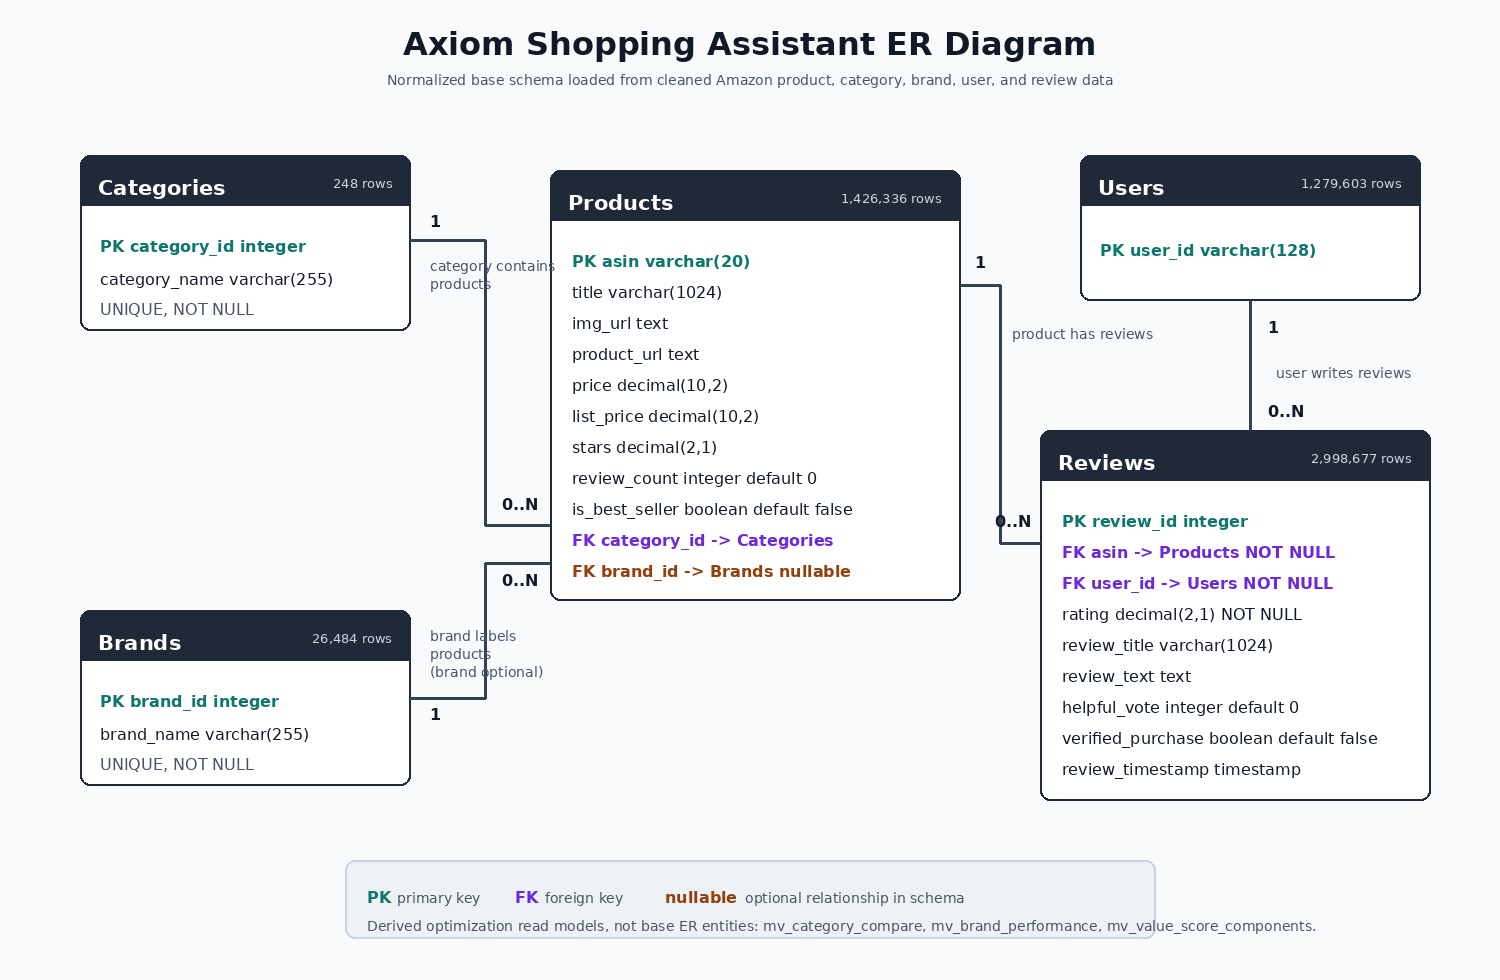
\includegraphics[width=0.92\linewidth]{er_diagram.png}
\end{center}

\subsection{3NF Proof}
\textbf{Categories.} \texttt{category\_id -> category\_name}; the determinant is
the primary key, and \texttt{category\_name} is unique.

\textbf{Brands.} \texttt{brand\_id -> brand\_name}; the determinant is the
primary key, and \texttt{brand\_name} is unique after canonicalization.

\textbf{Products.} ASIN determines title, image URL, product URL, price, list
price, stars, review count, best-seller flag, category ID, and brand ID. ASIN is
the primary key. Category and brand names are not stored redundantly on Products,
so there is no transitive dependency from ASIN through a foreign key to a
non-key display name.

\textbf{Users.} The only stored attribute is \texttt{user\_id}, which is the
primary key. There are no non-key attributes.

\textbf{Reviews.} Review ID determines the linked ASIN, user ID, rating, title,
text, helpful-vote count, verified-purchase flag, and timestamp. Product and
user details remain in Products and Users. The review fact table stores the
relationship and the review attributes only.

Every non-trivial functional dependency in the base schema has a superkey on the
left or a prime-attribute exception that does not arise here, so the design is
in 3NF. The materialized views used for optimization are derived read models,
not replacement base relations.

\section{Queries}
The Milestone 4 API Specification in \path{docs/reference/api_spec.pdf}
documented 15 routes: 12 query-backed primary routes and 3 auxiliary UI routes.
The final backend preserves those route contracts and now exposes 17 routes
across metadata, product browsing, product detail, cart, analytics, and ranking
workflows. The two public routes added after Milestone 4 are
\path{/products/category} and \path{/products/brand}; they support the final
Browse, Category, and Brand pages with paginated product lists, rating filters,
price filters, and stable URL state. The final implementation also adds
optional pagination/filter parameters where the UI needed them, the
\texttt{optimized} query-mode flag, and internal optimized SQL/helper queries
without changing the original Milestone 4 route names.

The report focuses on the most complex query families below, including the
post-Milestone-4 browse-list routes. Appendix A lists the final API catalog and
marks each route's Milestone 4 status. Appendix B maps query-backed behavior to
source files and calls out query families added after the API specification.

\small
\begin{longtable}{@{}L{0.23\linewidth}L{0.48\linewidth}L{0.23\linewidth}@{}}
\toprule
Route / feature & Query idea and application use & Complexity evidence \\
\midrule
\endhead
\path{/analytics/brands/performance} &
Computes brand-level product rating, best-seller count, linked-review count,
verified-review count, average review score, and helpful-vote total. Powers the
brand leaderboard. &
Brands/Products/Reviews joins, CTEs, grouping, HAVING-style filters, ordering. \\
\path{/analytics/reviews/trend} &
Groups reviews by month for a category and splits ratings by reviewer activity
group, exposing a credibility gap over time. &
Reviewer-count CTE, joins, \texttt{DATE\_TRUNC}, conditional aggregation. \\
\path{/products/trending} &
Ranks category products by recent linked review activity, using a data-relative
12-month window for the optimized default path. &
Review-horizon CTE, aggregation by ASIN, category/product/brand joins. \\
\path{/products/top-value} &
Finds products cheaper than their category average, rated above their category
average, and recently reviewed since the requested date. &
Correlated subqueries, EXISTS check, category/product joins, top-k ordering. \\
\path{/products/value-rankings} &
Normalizes rating, review count, price efficiency, and recent activity, then
combines them by user-selected weights. &
Multiple CTEs, global bounds, category bounds, aggregation, top-k score sorting. \\
\path{/products/:asin/helpful-reviews} &
Shows the target product's top reviews with reviewer-level context. &
Reviewer aggregate CTE in original path; optimized lateral aggregation over top reviews. \\
\path{/deals} &
Ranks discounted products by percentage off with price/rating filters. &
Expression sort, partial index opportunity, product/category join. \\
\path{/products/category}, \path{/products/brand} &
Return paginated category and brand product lists for the final browsing pages,
including rating and price filters plus display category/brand names. &
Product/category/brand joins, filter predicates, pagination, optimized CTEs that
page products before joining display names. \\
\bottomrule
\end{longtable}
\normalsize

\subsection{Milestone 4 API Reconciliation}
The API specification already covered search, deals, cart savings, product
detail side panels, analytics, trending, top-value, value rankings, and the
category/brand/product metadata helpers. During final frontend integration we
added two public browse-list routes, \path{/products/category} and
\path{/products/brand}, because search alone was not enough for stable category
and brand pages. These routes are backed by \texttt{categoryProductsQuery} and
\texttt{brandProductsQuery}, plus optimized variants, in
\path{server/queries/products/browse.sql.js}, exposed through
\texttt{api.categoryProducts} and \texttt{api.brandProducts} in
\path{client/src/api/client.js}, and used by the Browse, Category, and Brand
pages. Separately, the final \texttt{*QueryOptimized} exports and
materialized-view-backed SQL are post-Milestone-4 implementation additions used
by \texttt{?optimized=1}; they do not create new public endpoints. We also added
an internal \texttt{productExistsQuery} guard in
\path{server/queries/products/search.sql.js} so product-specific subroutes can
return clean 404 responses before running rating-distribution, helpful-review,
or alternatives SQL.

\section{Performance Evaluation and Optimization}
The benchmark runner executes one discarded warmup run, pauses for one second,
then records five measured \texttt{EXPLAIN ANALYZE} runs. The table reports
median execution time from the latest \texttt{docs/timings.md}. Representative
inputs are selected from the loaded database: the category with the most linked
reviews (\texttt{Toys \& Games}), an ASIN with more than 50 reviews
(\texttt{B0178IC734}), \texttt{reviewedSince=2018-01-01} for top-value, and the
Balanced \texttt{0.4/0.2/0.2/0.2} value-ranking weights.

\begin{center}
\small
\begin{tabularx}{\linewidth}{@{}L{0.17\linewidth}rrrY@{}}
\toprule
Query & Orig. ms & Opt. ms & Speedup & Main optimization \\
\midrule
Deals & 0.5 & 0.5 & 1.00x & Discount expression index already applied in current run \\
Category comparison & 3113.5 & 0.4 & 7962.92x & Materialized category summary \\
Top value & 324918.8 & 855.3 & 379.87x & Precomputed value components + MV index \\
Brand performance & 2366.2 & 3.7 & 643.68x & Materialized brand summary + sort index \\
Value rankings & 17047.1 & 1.4 & 12133.17x & Indexed default score in value MV \\
Trending & 1904.6 & 9.7 & 195.98x & Indexed recent-review count in value MV \\
Helpful reviews & 9118.3 & 7.1 & 1290.44x & Rank target reviews before reviewer stats \\
Review trend & 4601.9 & 4853.4 & 0.95x & Same SQL; route cache helps repeated reads \\
\bottomrule
\end{tabularx}
\normalsize
\end{center}

\subsection{Optimization Techniques}
\textbf{Indexing.} The schema includes foreign-key indexes, review timestamp and
ASIN indexes, category/brand product ordering indexes, a trigram index for title
search, and specialized materialized-view indexes such as
\path{idx_mv_value_components_default_score_cover}. A partial expression index
on \texttt{(1 - price/list\_price)} for valid discounted products keeps the
deals route sub-millisecond in the latest benchmark, while the largest measured
speedups now come from materialized category, brand, and value-summary paths.

\textbf{Materialized views.} \texttt{mv\_category\_compare},
\texttt{mv\_brand\_performance}, and \texttt{mv\_value\_score\_components}
precompute expensive aggregates and normalized dimensions. The value view stores
category price/rating averages, recent review counts, latest review timestamps,
normalized score components, and an indexed default Balanced score.

\textbf{Query restructuring.} The optimized helpful-review query first ranks the
target product's top ten reviews, then computes reviewer stats only for those
users. Category and brand listing queries page product rows before attaching
display names. Value ranking splits the default weighted case from custom
weights so the common Balanced preset can use the indexed precomputed score.

\textbf{Caching.} The backend uses a small in-memory TTL cache for optimized
category/brand metadata, optimized category comparison, and optimized review
trend by category. Brand performance is already backed by a small materialized
view and is returned without route-level caching to keep the code path simple.

\textbf{Why some optimizations are modest.} Some routes are already primary-key
or small-table lookups, so optimized and original timings are nearly identical.
The latest deals benchmark is also sub-millisecond in both branches because the
discount index benefits the current route shape. Review trend remains close
because the grouped SQL is already selective for the representative category;
route caching improves repeat users rather than the first
\texttt{EXPLAIN ANALYZE} timing.

\section{Robustness, Testing, and Code Quality}
The API validates malformed ASINs, missing required query parameters, invalid
numeric ranges, invalid dates, zero-sum ranking weights, and oversized cart
arrays. SQL uses parameterized bindings throughout. The client renders loading,
empty, and error states for API-backed pages and uses abortable fetches to avoid
stale UI updates after filters change.

The repository is split by responsibility: route modules, query modules,
database assets, data-pipeline scripts, client pages/components, and tests.
Server tests mock the database pool and cover validation, query selection,
caching, and response shape. Client tests cover API path building, routing,
cart behavior, pages, charts, formatting helpers, and the query-mode toggle.

\section{Technical Challenges}
\textbf{Product/review entity alignment.} The largest data challenge was joining
product ASINs with heterogeneous review sources. Some comment rows reference a
child ASIN, some use \texttt{parent\_asin}, and many raw reviews do not appear
in the product catalog. The cleaner handles both IDs, falls back to parent ASIN
when appropriate, and removes orphan reviews before ingestion.

\textbf{Brand entity resolution.} Product titles are noisy and the catalog has
no brand column. We used conservative title-prefix extraction, punctuation and
legal-suffix normalization, canonical display names, and a minimum five-product
threshold to avoid creating thousands of one-off brand entities.

\textbf{Large-file processing.} The full review sources are too large to clean
comfortably in memory. The pipeline streams review chunks, writes the review CSV
incrementally, and tracks users and duplicate keys while preserving stable
foreign-key relationships.

\textbf{Optimization tradeoffs.} Some rewritten SQL shapes were slower than the
planner's original choices. We therefore kept original variants for comparison,
used materialized views for aggregates that are stable between refreshes, and
only cached routes where repeat calls are common and the response changes
infrequently.

\section{Extra Credit and Tool Use}
Deployment extra credit is claimed for the hosted application configuration. The
frontend is configured with \texttt{VITE\_API\_BASE\_URL} set to
\url{https://team45-cis550-final-project.vercel.app}, and the backend CORS
allowlist is configured with \texttt{CLIENT\_ORIGIN} set to
\url{https://cis550-final-project.onrender.com}. The project also includes
substantial automated testing for robustness, and coverage can be measured with
the root and client coverage scripts.

Per the course plagiarism policy, generative AI was used to help with the
frontend's visual design direction and during final documentation and
consistency review to identify drift between the code, rubric, and writeups. The
team remains responsible for the project design, implementation, verification,
and final submitted content.

\appendix
\section{Appendix A: Final API Catalog}
\small
\begin{longtable}{@{}L{0.08\linewidth}L{0.22\linewidth}L{0.27\linewidth}L{0.23\linewidth}L{0.12\linewidth}@{}}
\toprule
Method & Path & Parameters & Response summary & M4 status \\
\midrule
\endhead
GET & \path{/categories} & Optional \texttt{optimized} & Category IDs and names & M4 aux \\
GET & \path{/brands} & Optional \texttt{optimized} & Brand IDs and names & M4 aux \\
GET & \path{/products/:asin} & Path ASIN, optional \texttt{optimized} & One product detail row & M4 aux \\
GET & \path{/products/search} & \texttt{keyword}, optional \texttt{minStars}, \texttt{limit}, \texttt{offset} & Product search rows & M4 query \\
GET & \path{/deals} & Optional \texttt{maxPrice}, \texttt{minStars}, \texttt{limit}, \texttt{offset} & Discount-ranked products & M4 query \\
GET & \path{/products/category} & \texttt{category}, optional filters/page params & Paginated category products & Post-M4 \\
GET & \path{/products/brand} & \texttt{brand}, optional filters/page params & Paginated brand products & Post-M4 \\
GET & \path{/products/:asin/rating-distribution} & Path ASIN & Five rating buckets and verified ratios & M4 query \\
GET & \path{/products/:asin/helpful-reviews} & Path ASIN & Top reviews with reviewer stats & M4 query \\
GET & \path{/products/:asin/alternatives} & Path ASIN & Cheaper, higher-rated alternatives & M4 query \\
POST & \path{/cart/savings} & JSON body \texttt{asins} & Aggregate list/current price and savings & M4 query \\
GET & \path{/analytics/categories/compare} & Optional \texttt{optimized} & Category aggregate metrics & M4 query \\
GET & \path{/products/trending} & \texttt{category}, optional \texttt{months} & Products ranked by recent reviews & M4 query \\
GET & \path{/products/top-value} & Optional \texttt{reviewedSince} & Above-average rating, below-average price products & M4 query \\
GET & \path{/analytics/brands/performance} & Optional \texttt{optimized} & Brand-level product/review metrics & M4 query \\
GET & \path{/analytics/reviews/trend} & \texttt{category}, optional \texttt{optimized} & Monthly review trend rows & M4 query \\
GET & \path{/products/value-rankings} & Optional \texttt{wRating}, \texttt{wReviews}, \texttt{wPriceEff}, \texttt{wRecent} & Weighted ranking rows & M4 query \\
\bottomrule
\end{longtable}
\normalsize

\section{Appendix B: Query Catalog and Source Files}
\small
\begin{longtable}{@{}L{0.21\linewidth}L{0.37\linewidth}L{0.23\linewidth}L{0.12\linewidth}@{}}
\toprule
Query family & Purpose & Source file & M4 status \\
\midrule
\endhead
Metadata lists & Category and brand selectors & \path{server/queries/meta.sql.js} & M4 aux \\
Product detail & Product overview by ASIN & \path{server/queries/meta.sql.js} & M4 aux \\
Product existence guard & Internal 404 check before product-specific subroutes & \path{server/queries/products/search.sql.js} & Post-M4 \\
Search & Keyword and minimum-star product search & \path{server/queries/products/search.sql.js} & M4 query \\
Deals & Discount ranking & \path{server/queries/products/deals.sql.js} & M4 query \\
Browse lists & Category and brand product pagination & \path{server/queries/products/browse.sql.js} & Post-M4 \\
Rating distribution & Per-star review histogram & \path{server/queries/products/detail.sql.js} & M4 query \\
Helpful reviews & Review snippets with reviewer context & \path{server/queries/products/detail.sql.js} & M4 query \\
Alternatives & Same-category cheaper and higher-rated products & \path{server/queries/products/detail.sql.js} & M4 query \\
Trending & Category products by recent review activity & \path{server/queries/products/trending.sql.js} & M4 query \\
Top value & Category-relative price/rating filter & \path{server/queries/products/value.sql.js} & M4 query \\
Value rankings & Weighted normalized score ranking & \path{server/queries/products/value.sql.js} & M4 query \\
Cart savings & Aggregate savings across selected ASINs & \path{server/queries/cart.sql.js} & M4 query \\
Category comparison & Category-level price, rating, and count & \path{server/queries/analytics.sql.js} & M4 query \\
Brand performance & Brand-level product and review aggregates & \path{server/queries/analytics.sql.js} & M4 query \\
Review trend & Monthly category review trends and credibility gap & \path{server/queries/analytics.sql.js} & M4 query \\
\bottomrule
\end{longtable}
\normalsize

\end{document}
